%\documentclass[10pt,preprint]{aastex}  % for e-submission to ApJ - one column
%\documentclass[12pt,preprint2]{aastex}  % for e-submission to ApJ - two column

\documentclass[iop,apjl, twocolappendix]{emulateapj}   % makes it look like the ApJ format

\pdfoutput=1

\usepackage{graphicx}
\usepackage{epsfig}
\usepackage{amsmath}
\usepackage{subfigure} 
%\usepackage{subcaption} 
\usepackage{comment}
\usepackage{hyperref}
\usepackage{amssymb}
\usepackage{apjfonts}
\usepackage{amsmath}
\usepackage{latexsym}
\usepackage{color}
\usepackage{algorithm}
\usepackage{algpseudocode}
\usepackage[usenames,dvipsnames,svgnames,table]{xcolor}
\usepackage{hyperref}
\usepackage[all]{hypcap}    %for going to the top of an image when a figure reference is clicked
\hypersetup{
	colorlinks,
		citecolor=blue,
		filecolor=blue,
		linkcolor=blue,
		urlcolor=blue
	}
\makeatletter
\algrenewcommand\ALG@beginalgorithmic{\ttfamily}
\makeatother

\newcommand{\red}[1]{\textcolor{red}{#1}}
\newcommand{\blue}[1]{\textcolor{blue}{#1}}
\newcommand{\green}[1]{\textcolor{green}{#1}}

\def\FG#1{{\textcolor{ForestGreen}{\textbf{\textit{ FG: #1}}}}}
\newcommand{\ENZO}{\textsc{ENZO}\xspace}


\shorttitle{Effect of AGN Thermal Heating with Radial Dependence on Thermal Stability of Simulated Galaxy Clusters}
\shortauthors{F. glines et al.}

\begin{document}
\title{Effect of Active Galactic Nuclei Thermal Heating with Radial Dependence on Thermal Stability of Simulated Galaxy Clusters}

\author{
  Forrest W. Glines \altaffilmark{1,2,3}, Brian W. O'Shea \altaffilmark{1,2}, G. Mark Voit\altaffilmark{1}
}

\affil{$^{1}${Department of Physics and Astronomy,
    Michigan State University, East Lansing, MI 48824, USA} }
\affil{$^{2}${Department of Computational Mathematics, Science and Engineering,
    Michigan State University, East Lansing, MI 48824, USA} }
\affil{$^{3}${\href{mailto:glinesfo@msu.edu}{glinesfo@msu.edu}}}

\label{firstpage}

\begin{abstract}
  \FG{Place holder abstract:}
  Observations from the last decade have revealed the existence of cool-core
  clusters, galaxy clusters with a cooling time  much shorter than the
  dynamical time. Recent work suggests that clusters may be thermally stable
  due a central heating mechanism such as an active galactic nucleus (AGN) that
  prevents cooling. Previous analytical work in one dimension has shown that
  thermal heating from a central AGN with a power-law radial profile, where the
  heating exceeds cooling at near and far radii but not in an intermediate
  region, may produce a stable cluster with an isentropic entropy profile in
  the core and an isothermal profile outside the cluster. To test this, we
  simulated idealized galaxy clusters using the ENZO code with thermal heating
  from a central AGN. Thermal heating as a function of radius was injected
  proportional to the radius to a fixed exponent in (-3,-2] for each run. Total
  thermal feedback was set equal to the total rate of cooling in the cluster.
  Thermal feedback with a conic angular dependence was also explored.  However,
  the purely thermal feedback was not enough to achieve thermal stability and
  each simulation collapsed due to overcooling. These simulation results
  support previous work showing that kinetic feedback through a jet in addition
  to thermal feedback is necessary for self-regulating AGN activity. 
\end{abstract}

\keywords{}

\section{Introduction}
\label{sec:introduction}

Most galaxy clusters in the universe have active galactic nuclei (AGN) at the
center of the cluster. These AGN play a significant role in the evolution of
the cluster, affecting the structure, quenching star formation, etc. \FG{References}

%\textbullet Cool-core problem and current resolution?
Feedback from AGN into the surrounding galaxy cluster has also been accepted as
the primary mechanism behind keeping cool-core clusters thermally stable in the
cool-core problem. Many galaxy clusters in the universe have been shown through
x-ray observations to have cooling times much shorter than the free-fall time.
Supernovae, star formation, and other effects are insufficient to heat the
cluster enough to prevent a cooling catastrophe and collapse. AGN, however, can
output enough energy through thermal and kinetic feedback to prevent the
collapse. Many recent simulations have shown that AGN activity triggered
through a number of mechanisms, including cold gas, can raise the core entropy
and prevent cooling.

\textbullet Constraints on AGN Feedback - self regulating?

\textbullet Elaborate on Voit analytical work - the toy model - a heating curve balancing
cooling that preserves the entropy profile

In cosmological simulations, AGN feedback is modeled using a subgrid process.
Due to the short timescale and small spatial scale evolution of the SMBH
comprising the AGN compared to the larger galaxy cluster, it is impossible to
coevolve the cluster and AGN simultaneously.

\textbullet AGN feedback in other simulations

Much recent work has been done to better physically motivate these subgrid
models to produce reasonable galaxy clusters. Triggering mechanisms explored
include ... The feedback back mechanism has also had a great effect on the
evolution of the cluster. Previous work by \cite{meece_jr_agn_2016} found that
for feedback near the cluster core a non zero kinetic feedback component was
needed to have a self regulating AGN; thermal heating alone in th e immediate
radius around the AGN was insufficient to keep the cluster thermally stable;

\textbullet \FG{Elaborate on Greg's work?}

This work  builds on \cite{meece_jr_agn_2016}, simplifying the feedback
mechanism by extending the radius of feedback to a much larger radius.


\textbullet Paper outline/roadmap

Galaxy clusters have predictable entropy profiles whose shape (although not
necessarily normalization) are mass-independent.
\cite{cavagnolo_intracluster_2009} Although -ray observations of the
intracluster medium (ICM) indicate that the central cooling times  in some
galaxy clusters are much shorter than the age of the universe, no cooling
catastrophe is observed. This argues that there is a heating mechanism that
offsets the cooling and acts on timescales comparable to the cooling time.
Given a variety of physical considerations, the primary heating source is
largely accepted to be active galactic nuclei (AGN).  What is not
well-understood, however, is the manner in which AGN deposit energy into the
ICM.   \textbf{The goal of this work} is to constrain the radial dependence of
the AGN energy injection by comparing a simplified model of AGN heating with
key X-ray observable quantities. This effort builds on work by Meece et. al.
\cite{meece_jr_agn_2016,meece_triggering_2017} using an idealized model of
thermal feedback over the cluster core following a power law, inspired by
analytical work by Voit et. al.
\cite{voit_global_2017}.

\section{Methodology}
\label{sec:methodology}

\subsection{AGN Feedback}
\textbullet Energy from the AGN is deposited as purely thermal energy in a
sphere encompassing the cluster.  The thermal feedback follows a power law with
radius, so that in general, $\dot{e} (r) \propto r^{-\alpha}$. However, this
led to several numerical challenges, including a feedback that asymtopes to
infinity at the AGN and a sharp cutoff in energy at the boundaries of the
simulation. These were overcome by adding a minimum radius smoothing length
$r_{\text{min}} = 1 \text{ kpc}$ (comprising \FG{FIXME} cells on the highest
refinement) and an exponential decay at a cutoff radius $r_c = 1 \text{ Mpc}.$
The full form of the feedback in $\text{ erg} \text{ s}^{-1} \text{ cm}^{-3}$ follows
\begin{equation}
  \dot{e}(r) = \frac{\dot{E}(t)}{A}
  \left\{\begin{matrix}
    \left( r_{\text{min}}/r_c \right )^{-\alpha} \exp {\left ( -r_{\text{min}}/r_c \right )} & , &r <= r_{\text{min}} \\
    \left( r /r_c \right )^{-\alpha} \exp { \left ( -r/r_c \right )}                         & , &r >  r_{\text{min}}
  \end{matrix}\right.,
\end{equation}
where $\dot{E}(t)$ is the total energy feedback from the energy at time $t$ and
$A$ is a scalar to normalize the feedback which is just the integral of the
feedback function over the entire feedback radius. Higher values of $\alpha$
correspond to more centralized feedback around the AGN. Without the inner
smoothing length, and $\alpha >= 3$ is unnormalizable, corresponding to
infinite energy feedback at the origin.

The total AGN heating rate $\dot E(t)$ tracks the total cooling rate within the
cluster, which is updated every $10 \text{ Myr}$ using \texttt{yt} to compute the total
X-ray cooling.

\textbullet Conic feedback. When the spherically symmetric feedback models
failed to maintain thermally stable galaxy clusters, we also investigated an
additional feedback model with a conic feedback. The conic feedback for $r >
r_{\text{min}}$followed
\begin{equation}
	\dot{e}(\theta) \propto \cos^2 \theta 
\end{equation}
where $\theta$ is the polar angle. Within $r <= r_{\text{min}}$, however, the
conic dependence was removed, as it would otherwise produce discontinuities
across the AGN. The normalization factor $A$ was also updated accordingly.

Energy from AGN feedback is deposited thermally in a sphere encompassing the
cluster. The deposited energy follows a power law:
\vspace{-0.5em}
\begin{equation}
	\dot{e}(r) \propto \left( \frac{r}{r_c} \right )^{-\alpha} \text{ erg} \text{ s}^{-1} \text{ cm}^{-3}.
	\vspace{-0.5em}
\end{equation}

\noindent
The thermal energy deposited in the cluster is scaled to exactly offset the
total cooling within the cluster, thus maintaining overall energy balance.
Simulations were run with a range of radial heating distributions ranging from
$\alpha = 2.0$ to 2.9. 
All simulations used the adaptive mesh code \texttt{Enzo}
\cite{bryan_enzo_2014-1} using AGN feedback algorithms modified from
\cite{meece_jr_agn_2016,meece_triggering_2017}.


We use a different $\alpha$ for each run, sampling from $2.0$ to
$2.9$ in $0.1$ increments and $2.5$ to $2.7$ in $0.05$ increments.

\subsection{Initial Conditions}
\label{sec:initial_conditions}
\textbullet Each simulation is run for $8 \text{Gyr}$, or approximately $4$
sound crossing times for the cluster. 

Simulations are initialized in a Perseus-like configuration, in the manner
of Meece \cite{meece_triggering_2017} and Li et al.\ \cite{li_cooling_2015} 

\section{Results}
\label{sec:results}

\begin{figure}
  \begin{center}
    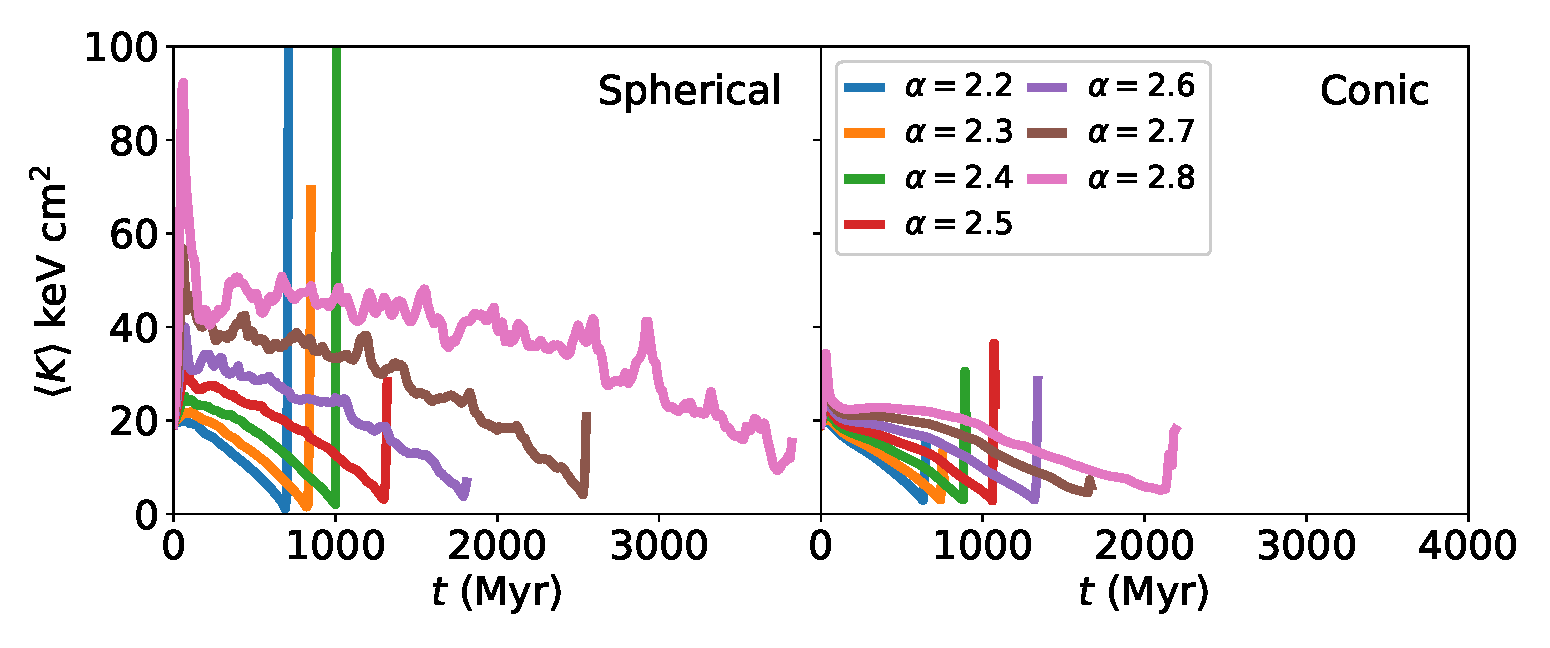
\includegraphics[width=1\linewidth]{figures/avgCoreEntropies.eps}
  \end{center}
  \caption{
    \label{fig:avgCoreEntropies}
    Mean entropy of the inner $10 \text{ kpc}$ proper as a function of time for
    simulations with radial exponents ranging from $\alpha=2.2$ to $\alpha=2.8$
    with spherical and conic feedback.  Mean entropy is calculated by the
    mass-weighted temperature and the volume-weighted density. To improve
    visibility, these are plotted up until $30 \text{ Myr}$ after the mean core
    entropy has increased by $60\%$ in a $10 \text{ Myr}$ span, or until the
    simulation has stopped. After this point, the entropy profile has diverged
    from what would be expected from observations. Simulations using values of
    $\alpha$ between those shown here were also run, although all exhibited the
    same core entropy decay with higher values of $\alpha$ decaying slower and
    conic feedback collapsing faster.
  }
\end{figure}

Feedback failed to self regulate nor preserve thermal stability.
Fig. \ref{fig:avgCoreEntropies} shows the mean core entropy of the inner $10
\text{ kpc}$ as a function of time for several representative simulations. For
all choices of $\alpha$ with either spherical or conic feedback, the core
entropy slowly dropped over time until a clump of cold gas formed, at which
point each simulation then went through a cooling collapse. As the total
cooling in the cluster spiked, the AGN activity also spiked. If the simulation
was able to continue through the collapse and AGN outburst, the subsequent
cluster was left with an unphysically high entropy profile, as is shown in the
entropy phase plots in fig. \ref{fig:phasePlots}.

High values of $\alpha$, or more centrally peaked feedback, led the collapse to
happen later. Although even higher values of $\alpha$ may prevent the collapse
for longer, the central heating asymptotes to infinity as $\alpha \rightarrow
3$. A simulation with $\alpha=2.9$ led to immediate discontinuities in the
fluid that the hydrodynamics solvers were unable evolve. \FG{Need to elaborate
on this?} Additionally, the higher $\alpha$ runs led to central entropies and
surface brightnesses that are unreasonable from observations (see figs.
\ref{fig:allVradius} and \ref{fig:allValpha}.)

\FG{Make a footnote? Include in each plot?} Most plots in this section are
taken at $t = 500 \text{ Myr}$, an arbitrary time step after the initial
settling of the cluster and before collapse which demonstrates the approximate
structure of each simulation. Before $t=500 \text{ Myr}$ the higher $\alpha$
runs have not settled from the initial burst AGN activity while later than
$t=500 \text{ Myr}$ the lower $\alpha$ simulations have already collapsed. The
two $\alpha$ values $2.2$ and $2.8$ are used as the most extreme values of
$\alpha$ simulated that evolved to $t= 500 \text{ Myr}$ without collapsing.

\begin{figure*}
	\begin{center}
    \includegraphics[width=1\linewidth]{figures/radius_entropy_profiles}
		\includegraphics[width=1\linewidth]{figures/radius_cooling_rate_profiles}
	\end{center}
	\caption{
    \label{fig:profiles}
    Phase plots of entropy and cooling rate versus radius of simulations with
    spherical and conic AGN heating with radial exponents $\alpha=2.2$ and
    $\alpha=2.8$ as labeled, with the initial and current median entropy or
    cooling rate versus radius in dashed blue and solid black respectively. The
    total heating rate in a shell versus radius is superimposed on the cooling
    rate in solid red, which is scaled in the simulation to match in total
    cooling rate.  The upper plots are at $t= 500 \text{ Myr}$
    and the lower plots are at the final time step of the simulation.
    \FG{Should I include the final step? Maybe more a time sequence through
    collapse of one simulation? Combine r axes. Also, maybe a radial profile of
    cold gas to see where it forms}}
\end{figure*}

Fig. \ref{fig:profiles} shows phase plots of entropy and the cooling rate
versus radius. As expected, at $t= 500 \text{ Myr}$ the higher $\alpha=2.8$ run
has a higher core entropy than $\alpha=2.2$ since more energy is deposited in
the center. The median entropy profile still follows the initial median but
there is more high entropy gas near the core. Both the spherical and conic
$\alpha=2.2$ evolved past their collapse but are left with core entropy
profiles too high to match observations. The $\alpha=2.8$ simulations formed
cold gas near their cores as they collapsed before hydrodynamic errors stopped
the simulations.
The heating rate is also plotted with the median cooling in the cooling rate
phase diagram. For certain values of $\alpha$, heating exceeds cooling in the
inner core and outer radii but not in the intermediate range where the entropy
profile changes from a flat line to a power law. \FG{This would make more
sense with volume averaged cooling rate instead of the median - that's what
should be directly compared.} However, this criterion was not enough to produce
thermally stable clusters.

\begin{figure}
	\begin{center}
		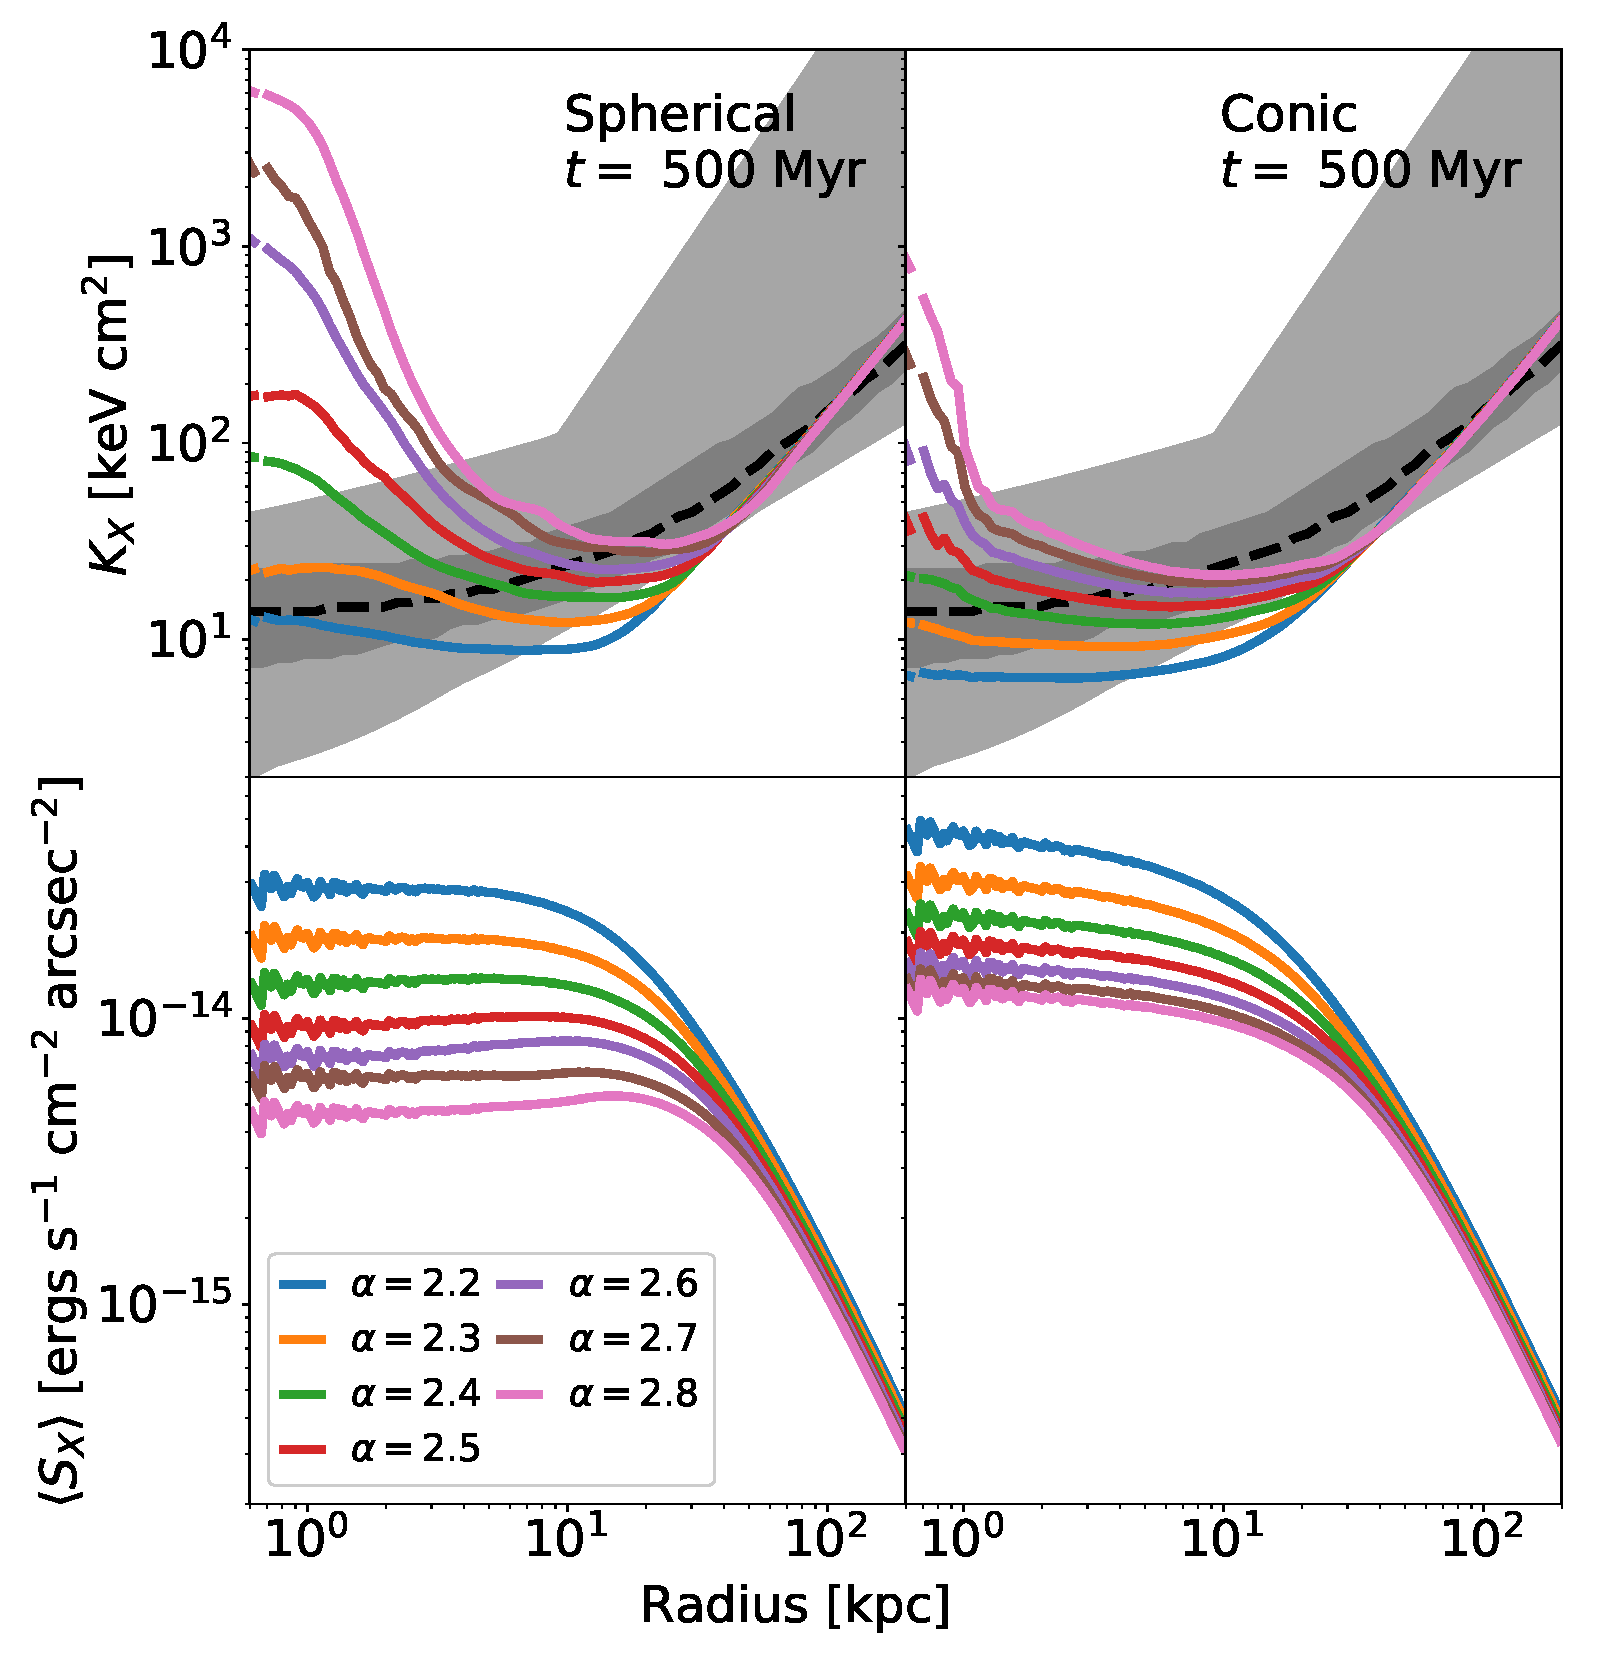
\includegraphics[width=1\linewidth]{figures/allVradius.eps}
	\end{center}
	\caption{
    \label{fig:allVradius}
    \textbf{Top:} Mean entropy as a function of spherical radius from
    several representative simulations using different radial exponents
    $\alpha$ for heating with spherical feedback (left) and conic feedback
    (right.) Mean entropy is calculated by the mass-weighted temperature and the
    volume-weighted density.
    \textbf{Bottom:}Mean simulated X-ray surface brightness in the $0.5 -2.0
    \text{ keV}$ band as a function of observing radius from several
    representative simulations using different radial exponents $\alpha$ for
    heating with spherical feedback (left) and conic feedback (right.) All data
    is taken at $t= 500 \text{ Myr}$. \FG{Add density? Add text annotations?
    Combine with fig. \ref{fig:allValpha}? Combine spherical and conic onto one
    plot?}
  }
\end{figure}

Fig. \ref{fig:allVradius} shows the entropy and surface brightness profiles of
several simulations at $t=500 \text{ Myr}$ with both spherical and conic
feedback. High $\alpha$ and so more centralized feedback lead to elevated core
entropies that slope up and away from the initial flat entropy core. The lower
$\alpha$ simulations with more realistic entropy profiles \FG{(realistic?)},
however, collapse soon after reaching a flat core entropy. The lower surface
brightness is likely due to the lower density in the core.

\begin{figure}
	\begin{center}
		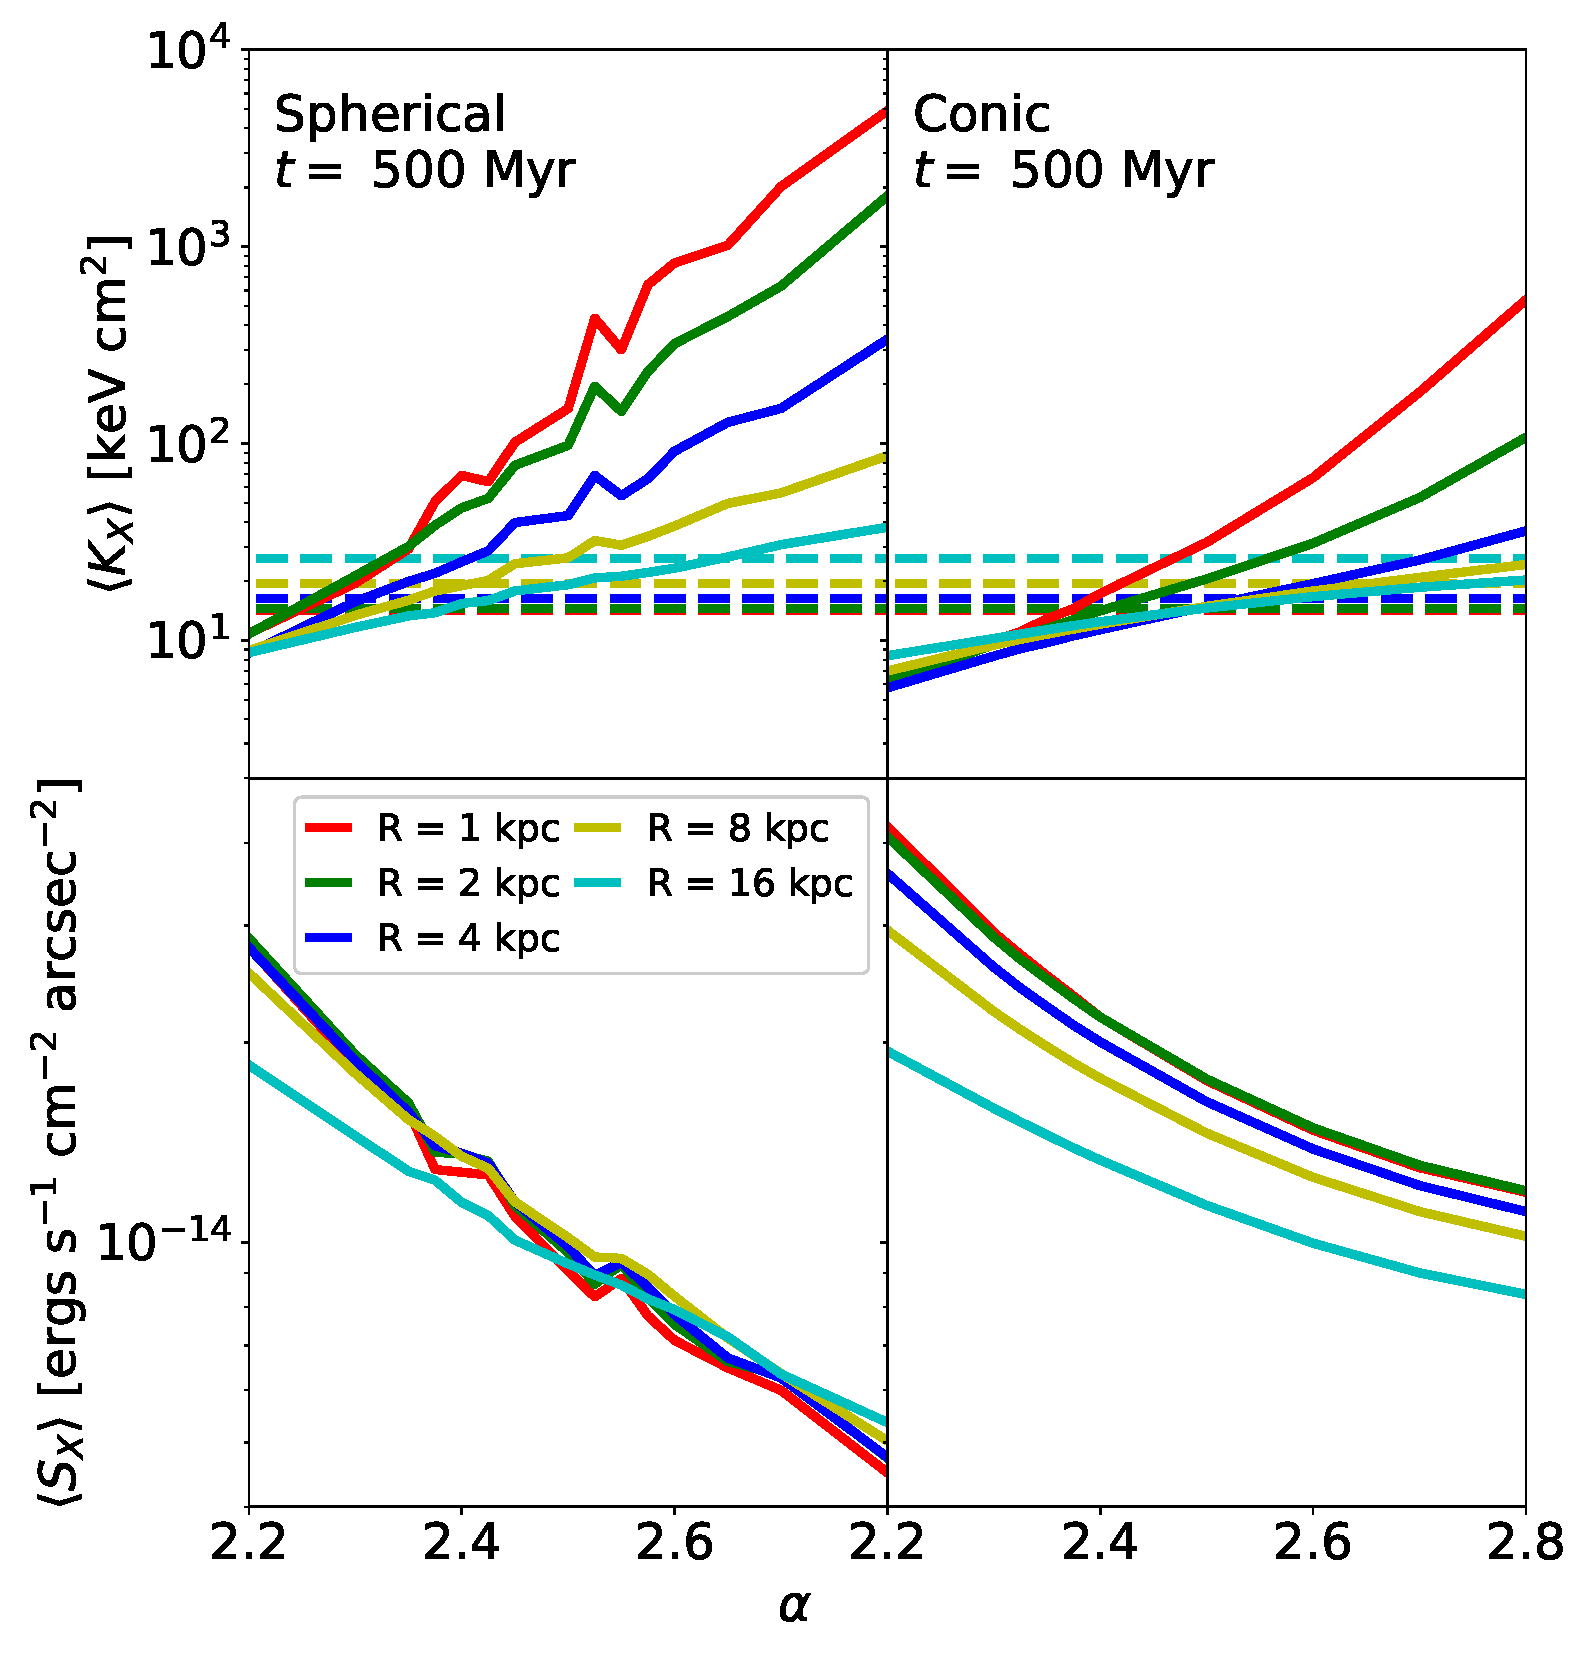
\includegraphics[width=1\linewidth]{figures/allValpha.eps}
	\end{center}
	\caption{
    \label{fig:allValpha}
    \textbf{Top:}  Mean cluster core entropy calculated within impact
    parameters ranging from $R = 2^0 - 2^4$ proper kpc as a function of
    $\alpha$ for heating with spherical feedback (left) and conic feedback
    (right.) Mean entropy is calculated by the mass-weighted temperature and the
    volume-weighted density.
    \textbf{Bottom:}	Mean simulated X-ray surface brightness in the $0.5 - 2.0
    \text{keV}$ band of cores of radii $R = 2^0 - 2^4$ proper kpc from as a
    function of $\alpha$ for heating with spherical feedback (left) and conic
    feedback (right.) All data is take at $t= 500 \text{ Myr}$.}
\end{figure}

As expected, core entropy increases with $\alpha$ in fig. \ref{fig:allValpha}
due to the higher amount of energy deposited in the core. The core surface
brightness diminishes with $\alpha$, partly due to lower cooling rates and less
massive cores as higher $\alpha$ pushes more mass out of the core. From
examining different core sizes, the effect of different $\alpha$ is more
visible for smaller cores for larger $\alpha$. Note that the total heating in
the core scales greater than linearly with $\alpha$ \FG{Check how this scales:
is it exponentially?}.

\begin{figure*}
	\begin{center}
		\includegraphics[width=0.49\linewidth]{figures/entropy_slices}
		\includegraphics[width=0.49\linewidth]{figures/density_slices}
		\includegraphics[width=0.49\linewidth]{figures/temperature_slices}
		\includegraphics[width=0.49\linewidth]{figures/cooling_rate_slices}
	\end{center}
	\caption{
    \label{fig:slices}
    Slices of entropy, density, temperature, and cooling rate through the
    origin of simulations with spherical and conic AGN heating with radial
    exponents $\alpha=2.2$ and $\alpha=2.8$ as labeled. All data is taken at
    $t= 500 \text{ Myr}$. \FG{Are these figures worth including? Combine x and y axes?}}
\end{figure*}

Fig. \ref{fig:slices} shows slices through the origin of the entropy, density,
temperature, and cooling rate of simulations with spherical and conic heating
with $\alpha=2.2$ and $\alpha=2.8$, two more extreme values of $\alpha$. In
both high $\alpha$ simulations, the core entropy and temperature are raised
while the core density and cooling rate is lower. In the conic simulations, the
jet structure is more apparent in high $\alpha$ cases. The jet is also more
collimated than would be expected for the $\cos^2 \theta$ dependence used,
although this may be due to the small radius where the majority of the energy
is deposited in the high $\alpha$ case.

\begin{comment}
\begin{figure}
  \caption{Cold gas fraction as a function of time}
\end{figure}
\end{comment}

\section{Discussion}
\label{sec:discussion}

\textbullet Higher energy input into core leads to slower collapse times, larger flat entropy cores.

\textbullet Formation of multiphase gas leads to collapse?

Higher $\alpha$, corresponding to more energy input at the cluster core,
predictably raised core entropy. Lower $\alpha$ left a flat entropy
profiles closer to the initial conditions.  The higher $\alpha$
simulations push out enough gas from the core to decrease x-ray
brightness. 

Although this is a very simplified model of cluster feedback, it can be used to
constrain the broad properties of AGN feedback -- in particular, the radial
dependence of its heat deposition -- using X-ray observations.  In the near
future, we will make direct comparisons to Chandra X-ray data of entropy and
surface brightness profiles  using the ACCEPT survey
\cite{cavagnolo_intracluster_2009} and its successors.

\section{Summary}
\label{sec:summary}

\begin{itemize}
  \item No configuration of radial exponent $\alpha$ for purely thermal feedback with
    spherical nor conic feedback achieved thermal stability; all simulations
    collapsed during the formation of cold gas.
  \item Higher values of $\alpha$, corresponding to more centralized feedback,
    increased core entropy, lowered core surface brightness, and delayed
    collapse. Conic feedback also hastened collapse.
\end{itemize}

\acknowledgments
\section{Acknowledgments}
\label{sec:acknowledgments}
This project has been supported by NASA through Astrophysics Theory Program
grant \#NNX15AP39G and Hubble Theory Grant HST-AR-13261.01-A, and by the
NSF through grant AST-1514700.  The simulations were run on the NASA
Pleiades supercomputer through allocation SMD-16-7720.  \texttt{Enzo} and
\texttt{yt} are developed by a large number of independent researchers from
numerous institutions around the world. Their commitment to open science
has helped make this work possible.

%\input{apj-bib}
\bibliographystyle{apj}

\bibliography{apj-jour,AGNThermal2018}

\end{document}
